\documentclass[25pt,halfparskip-,pagesize]{scrartcl}
\usepackage[papersize={34in,44in},body={780mm,1000mm},top=.5in,ignoreheadfoot]{geometry}
\usepackage{eso-pic}
%\usepackage{bera}
%\usepackage{fourier}
%\usepackage[scaled]{luximono}
\usepackage[T1]{fontenc}
\usepackage[english]{babel}
\usepackage{graphicx,color,multicol,booktabs,listings,fancybox,calc}
\usepackage{capt-of}
\usepackage{subfigure}
%\raggedcolumns
\flushcolumns

%\show\hrulefill
\AddToShipoutPicture{%
    \AtPageUpperLeft{\makebox(0,0)[lt]{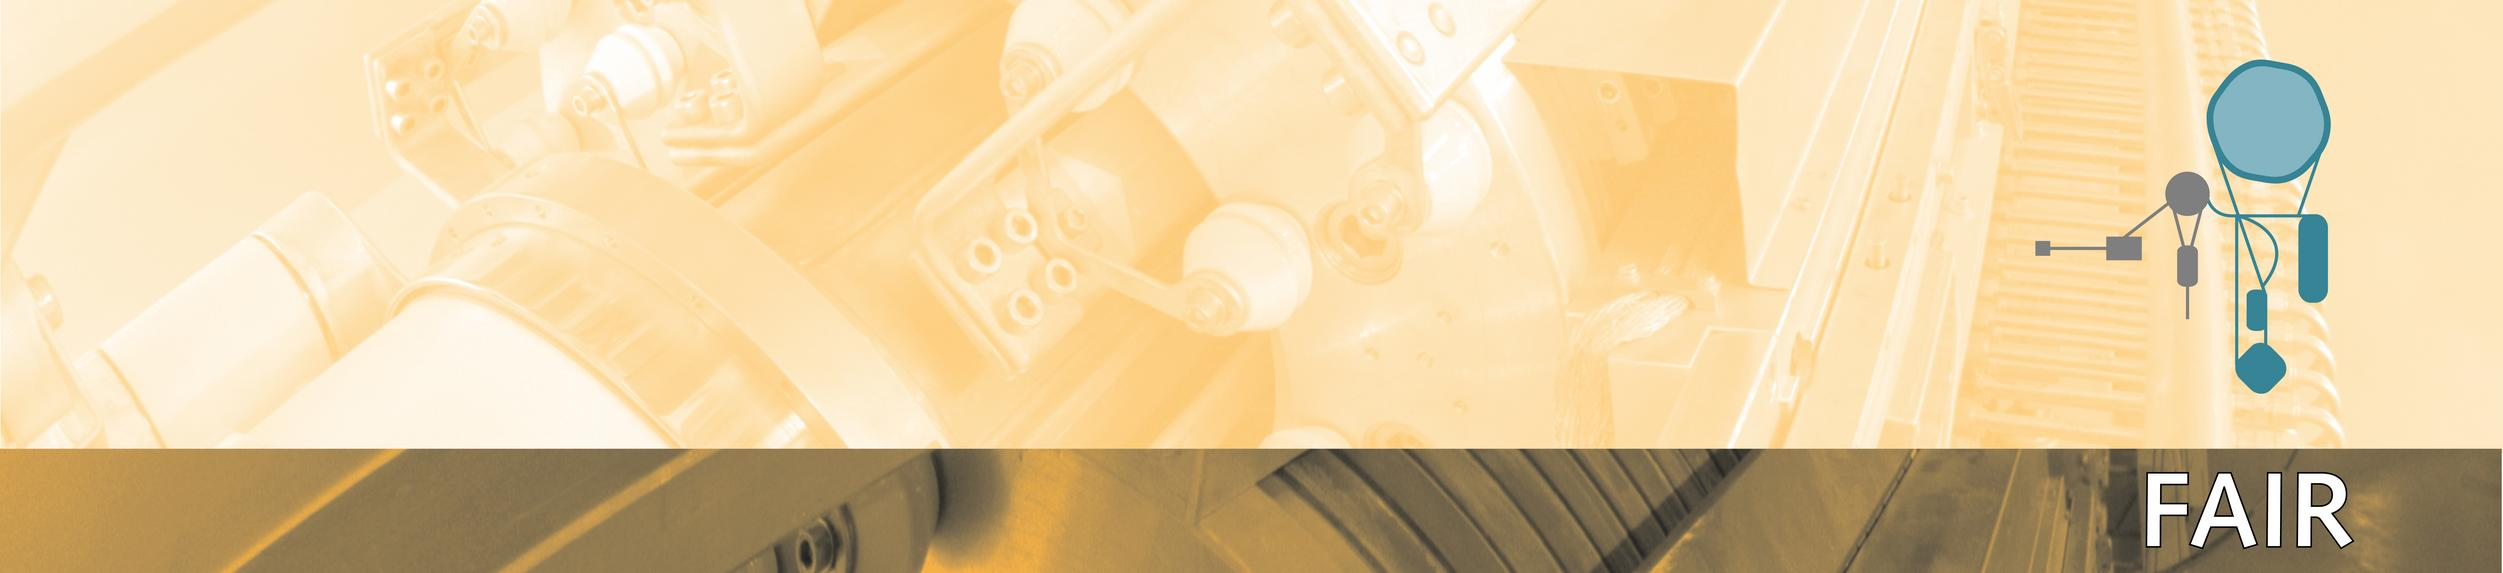
\includegraphics[width=\paperwidth]{head-small}}}
    \unitlength1cm
    \AtPageUpperLeft{\kern5cm\lower9cm\hbox{
\includegraphics[width=11cm]{../images/GSI_Logo_cmyk.eps}}}
    \AtPageUpperLeft{\kern.1cm\rule[-.3cm]{.4pt}{.2cm}}
    \AtPageUpperLeft{\kern.1cm\rule[-.1cm]{.2cm}{.4pt}}
    \AtPageUpperLeft{\kern\paperwidth\kern-.1cm\rule[-.3cm]{.4pt}{.2cm}}
    \AtPageUpperLeft{\kern\paperwidth\kern-.3cm\rule[-.1cm]{.2cm}{.4pt}}
    \AtPageLowerLeft{\kern.1cm\rule[.1cm]{.4pt}{.2cm}}
    \AtPageLowerLeft{\kern.1cm\rule[.1cm]{.2cm}{.4pt}}
    \AtPageLowerLeft{\kern\paperwidth\kern-.1cm\rule[.1cm]{.4pt}{.2cm}}
    \AtPageLowerLeft{\kern\paperwidth\kern-.3cm\rule[.1cm]{.2cm}{.4pt}}
    \linewidth2pt
    \AtPageLowerLeft{\kern1in\kern\oddsidemargin\lower-3cm\hbox to \textwidth{\leaders \hrule height \linewidth \hfill \kern 1cm\lower.5cm\hbox{
\includegraphics[height=2cm]{../images/GSI_Logo_cmyk.eps}}\kern1cm\rule{3cm}{\linewidth}}}
    \AtPageLowerLeft{\kern1in\kern\oddsidemargin\lower-2cm\hbox{\sffamily\fontsize{12pt}{12pt}\selectfont ICALEPCS\,2011}}
}

\def\TTra{\textsuperscript{\texttrademark}}
\definecolor{title}{cmyk}{.00,0.15,0.75,0}
\definecolor{solution}{cmyk}{.10,1.00,.80,0}
%\definecolor{colsection}{cmyk}{1,.8,0,0}
\definecolor{colsection}{cmyk}{0,.6,.6,.7}
\definecolor{itemgreen}{cmyk}{1,0,.9,.2}
\definecolor{itemroyalblue}{cmyk}{.711,.533,0,.118}
\definecolor{itemblue}{cmyk}{1,1,0,.2}
\definecolor{lstbackground}{cmyk}{0.35,0.05,0.0,0.0}
\definecolor{lstemph}{cmyk}{0.0,1.0,0.95,0.0}
\definecolor{lstbackgroundalt}{cmyk}{0.05,0.05,0,0.2}
\definecolor{lststring}{cmyk}{.6,1,.8,0}
\newcommand{\solution}[1]{\textbf{\textcolor{solution}{#1}}}
\setkomafont{descriptionlabel}{\itshape}
\setcounter{secnumdepth}{-1}
\pagestyle{empty}
\addtokomafont{section}{\color{colsection}}
\addtokomafont{caption}{\itshape}
\setlength{\columnsep}{5em}
\newcommand\mycaption[1]{\textit{#1}}
%\renewcommand{\familydefault}{\rmdefault}

\usepackage{pifont}
\renewcommand*\labelitemi{\color{colsection}\ding{110}}
\renewcommand*\labelitemii{\color{itemgreen}\ding{108}}

\lstset{showstringspaces=false,basicstyle=\ttfamily\small,
    keywordstyle={\bfseries},stringstyle={\color{lststring}},tabsize=4,framerule=2pt,rulecolor=\color{black},
    rulesep=5pt,abovecaptionskip=6pt,belowcaptionskip=8pt,
    emphstyle=\color{lstemph}}

\lstdefinelanguage{nodal}
}

\newcommand\class[1]{\texttt{#1}}

\makeatletter
\DeclareRobustCommand{\Cpp}
{\valign{\vfil\hbox{##}\vfil\cr
   C\kern-.05em\cr
      %$\hbox{\fontsize{\sf@size}{0}+\kern-0.05em+}$\cr}%
      \hbox{+\kern-0.05em+}\cr}%
}
\makeatother

\setlength{\fboxsep}{1em}
\raggedright
\begin{document}
\vspace*{1ex}

{\centering
\begin{minipage}{20in}
\centering \sffamily\Huge \rule{0pt}{50pt}\textbf{Facility-Wide Synchronization of Standard FAIR Equipment Controllers}\par
\vspace{5mm} \LARGE S. Rauch,
W. Terpstra,
W. Panschow,
M. Thieme,
C. Prados,
M. Zweig,
M. Kreider,
D. Beck,
R. B\"ar
\par
\vspace{5mm}
\Large GSI, D-64291 Darmstadt, Germany
\rule[-12pt]{0pt}{10pt}\par
\end{minipage}%
\par}%

\vspace{11cm}
\setlength{\fboxrule}{1pt}
\begin{multicols*}{3}
\ovalbox{%
\begin{minipage}{\linewidth}
\section{Abstract}
\small The standard equipment controller under development for the new FAIR
accelerator facility is the Scalable Control Unit (SCU). It is designed to
synchronize and control the actions of up to 12 purpose-built slave cards,
connected in a proprietary crate by a parallel backplane. Inter-crate
coordination and facility-wide synchronization are a core FAIR requirement
and thus precise timing of SCU slave actions is of vital importance.

The SCU consists primarily of two components, an x86 COM Express daughter
board and a carrier board with an Altera Arria II GX FPGA, interconnected by
PCI Express. The x86 receives configuration and set values with which it
programs the real-time event-condition-action (ECA) unit in the FPGA. The
ECA unit receives event messages via the timing network, which also
synchronizes the clocks of all SCUs in the facility using White Rabbit.
Matching events trigger actions on the SCU slave cards such as: ramping
magnets, triggering kickers, etc.

Timing requirements differ depending on the action taken. For softer
real-time actions, an interrupt can be generated for complex processing on
the x86. Alternatively, the FPGA can directly fire a pulse out a LEMO output
or an immediate SCU bus operation. The delay and synchronization achievable
in each case differs and this paper examines the timing performance of each
to determine which approach is appropriate for the required actions.
\par
\end{minipage}}



%\par
%\vfill

\section{Introduction}
\begin{itemize}
	\item 2x EIA-232
\end{itemize}
In the FAIR control system,
a data master issues high-level commands to control accelerator devices.
The front-end controllers in the system react to relevant commands,
issuing appropriate actions to their hardware components.
Depending on the action to be taken,
there are different timing requirements to be met.

Unlike the control system currently deployed at GSI,
commands issued by the data master carry an absolute execution timestamp.
The front-end controllers must receive commands early enough
that they can schedule their actions
to achieve the desired result at the correct time.
Unfortunately, executing actions takes a variable amount of time.
If the action takes 90-110$\mu$s to execute,
then this places two constraints on the system.
Firstly, the data master must issue commands at least 110$\mu$s ahead of time.
Secondly, the system must be able to tolerate that the action could be as
much as 10$\mu$s too early or too late.


Issuing commands too far in advance reduces the responsiveness of the system.
Once the data master has issued a command, it cannot be aborted.
If the situation changes,
perhaps due to interlock or contention from another beam user,
the system cannot react faster than the slowest action already executing.
This neglects, of course, other sources of latency in the system,
such as network propagation delay, which only exacerbate the problem.
It is thus generally desirable to have fast action execution.

Non-deterministic execution time is a potentially much more serious problem.
For example, if a kicker executes an action a few nanoseconds too late,
the beam might be lost.
However, not all actions require the same precision,
and it may make sense to trade accuracy for flexibility in some situations.

Fortunately, the  most common equipment controller in FAIR,
the Scalable Control Unit (SCU),
has several possibilities for executing actions.
This paper outlines the timing requirements of various accelerator
components in FAIR and explorers the alternatives which could meet them.



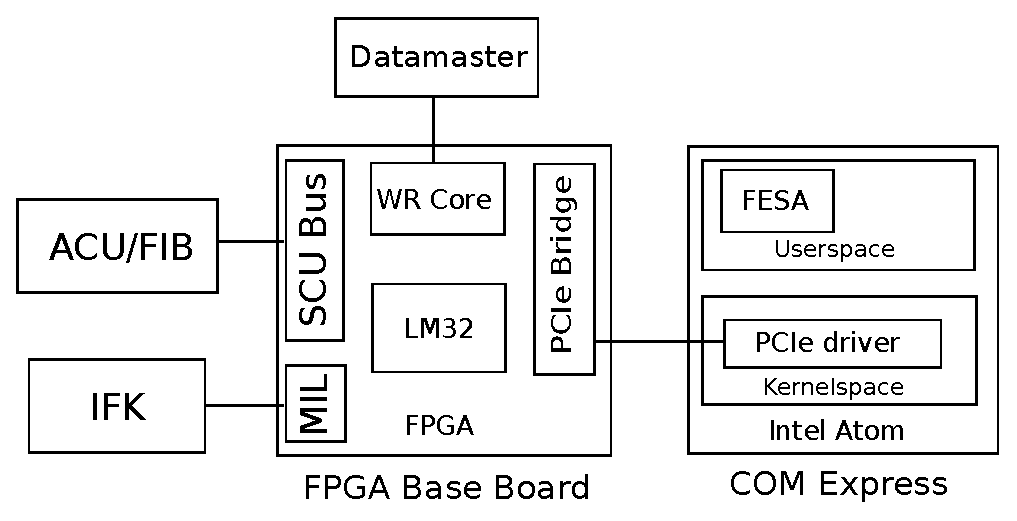
\includegraphics[width=\columnwidth]{../images/WEPD48f2}
\captionof{figure}{Block diagram of SCU}

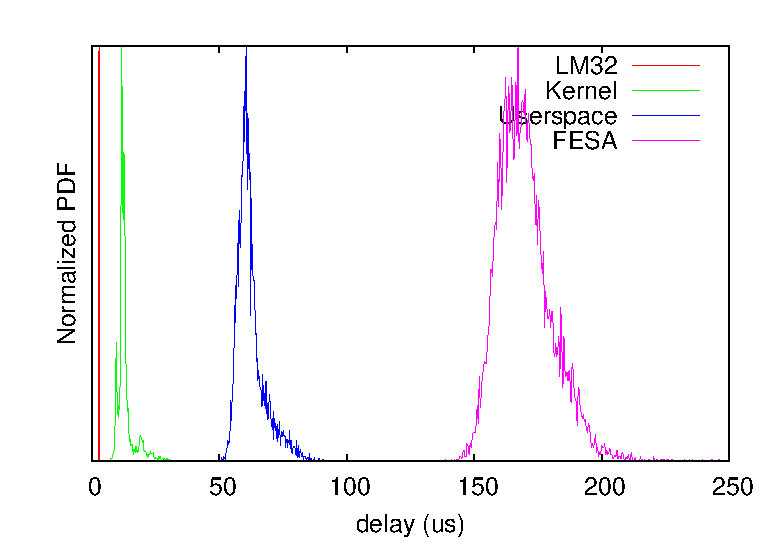
\includegraphics[width=\columnwidth]{../images/WEPD48f1}
\captionof{figure}{Comparison of delay distributions}

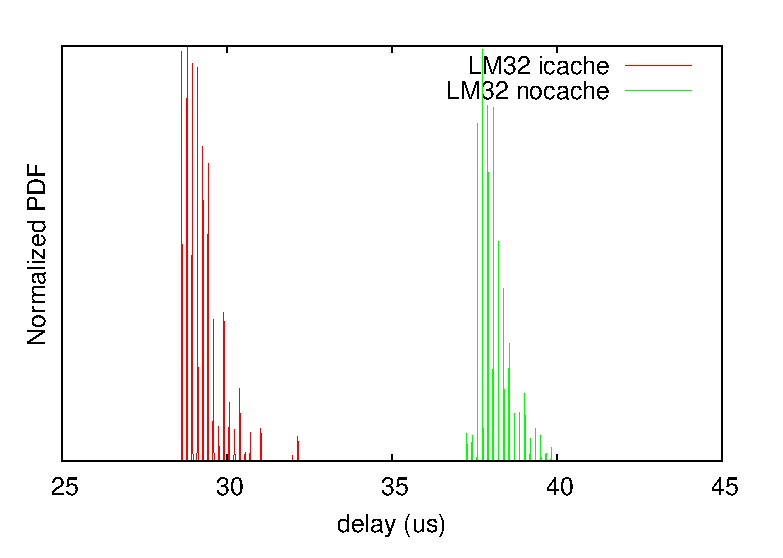
\includegraphics[width=\columnwidth]{../images/lm32plot}
\captionof{figure}{LM32 delay distribution}

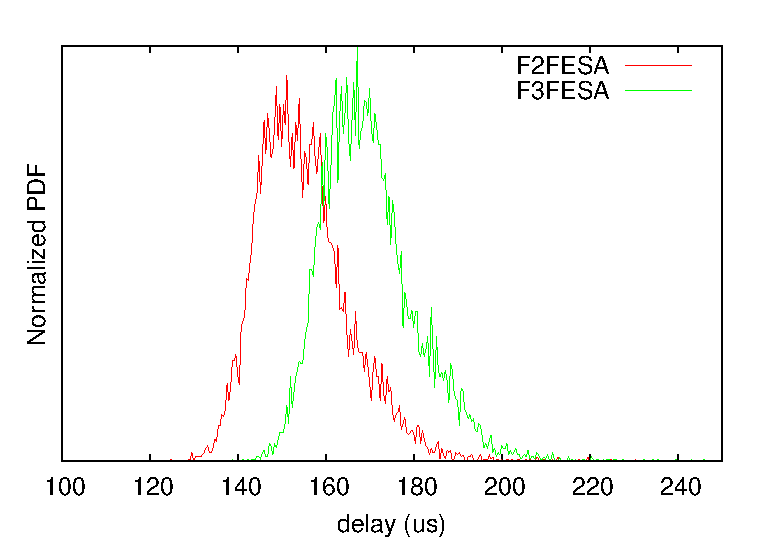
\includegraphics[width=\columnwidth]{../images/fesa_plot}
\captionof{figure}{FESA delay distribition}

%\begin{figure}[t]
%   \centering
   \begin{tabular}{l|c|c|c|c}
     $\mu$s    & min   & mean  & max   & stddev \\
     \hline
     FPGA      & 0 & 0.001 & 0.001 & 0.001 \\
     LM32      & 2.863 & 2.924 & 3.217 & 0.058  \\
     Kernel    & 7.120 & 13.29 & 37.73 & 3.49   \\
     Userspace & 49.36 & 62.49 & 93.33 & 5.62   \\
     FESA      & 138.9 & 170.1 & 246.1 & 10.8 \\
   \end{tabular}
   \caption{Execution timing performance}
  \label{tab:stat_table}
%\end{figure}



%\begin{figure}
%\subfigure[Bildunterschrift]{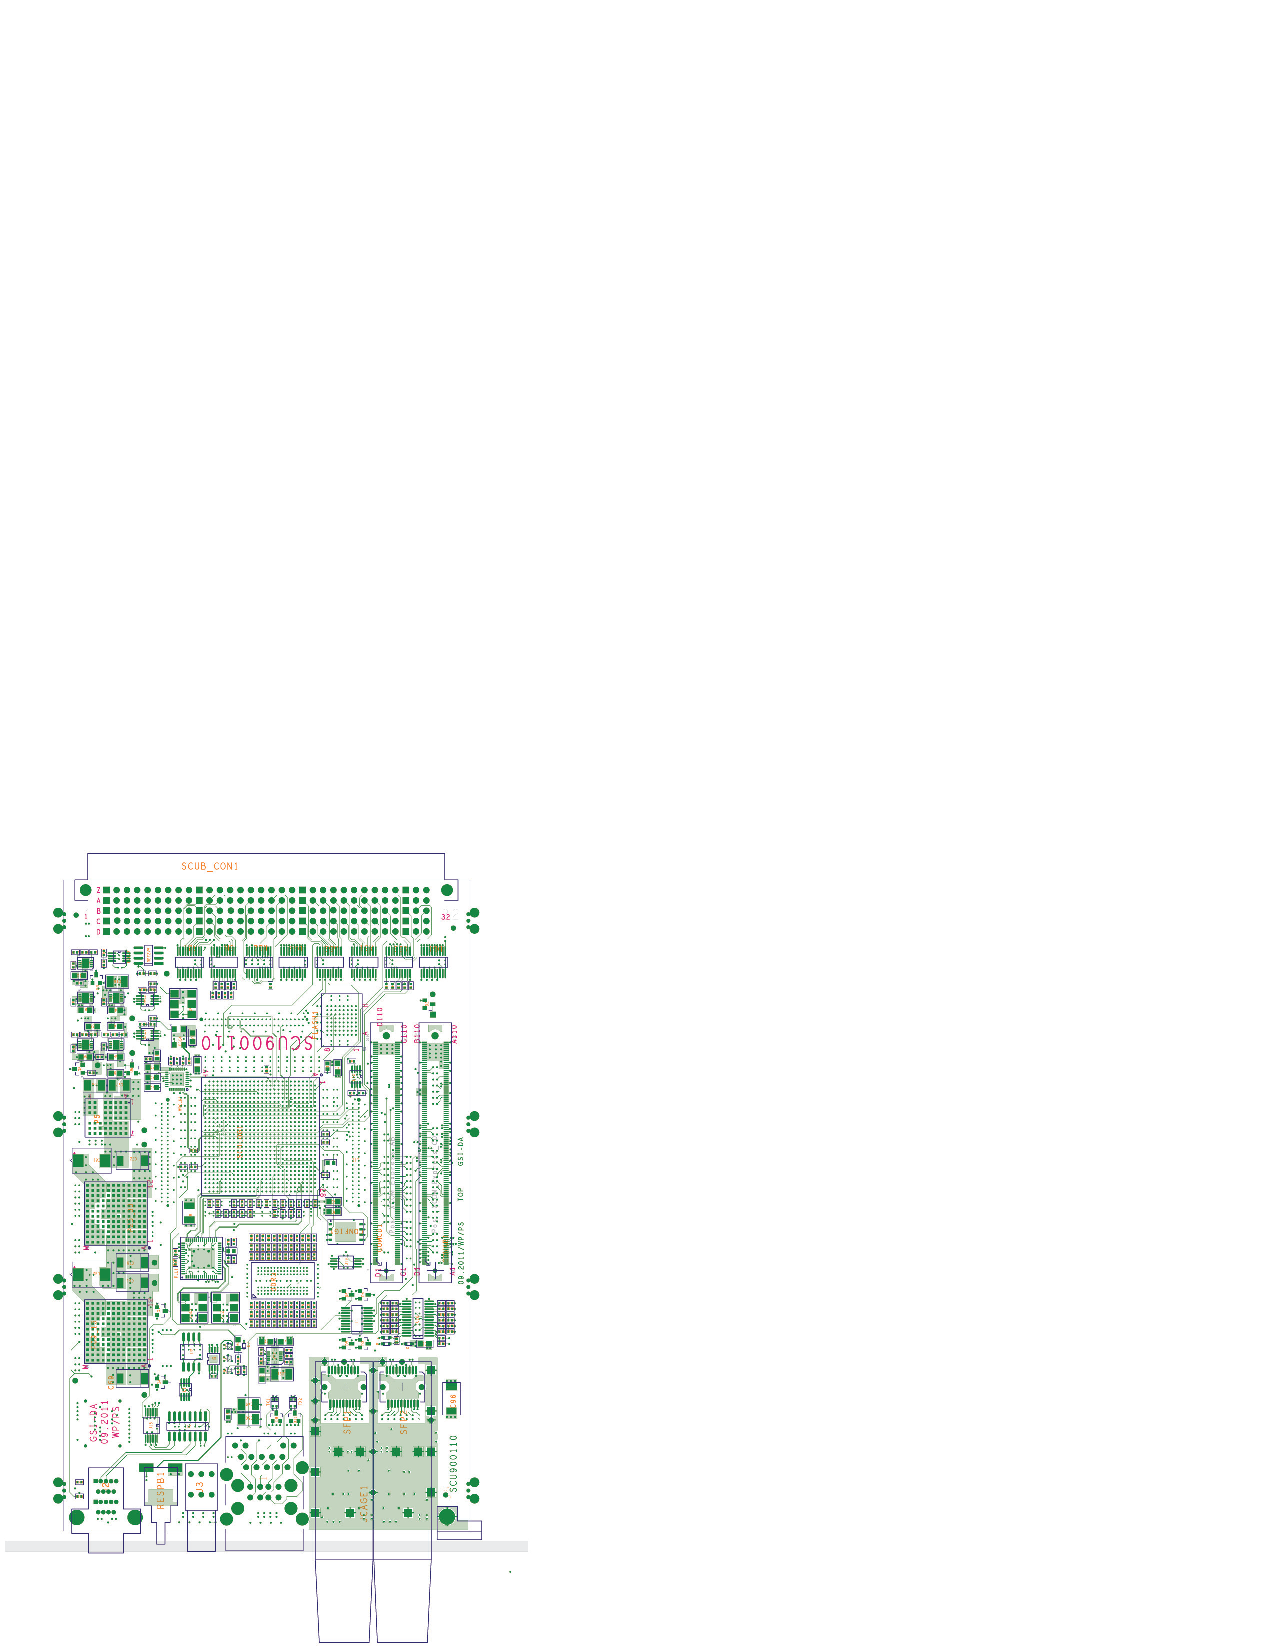
\includegraphics[width=0.49\columnwidth]{../images/WEPMN018f2}}\hfill
%\subfigure[Bildunterschrift]{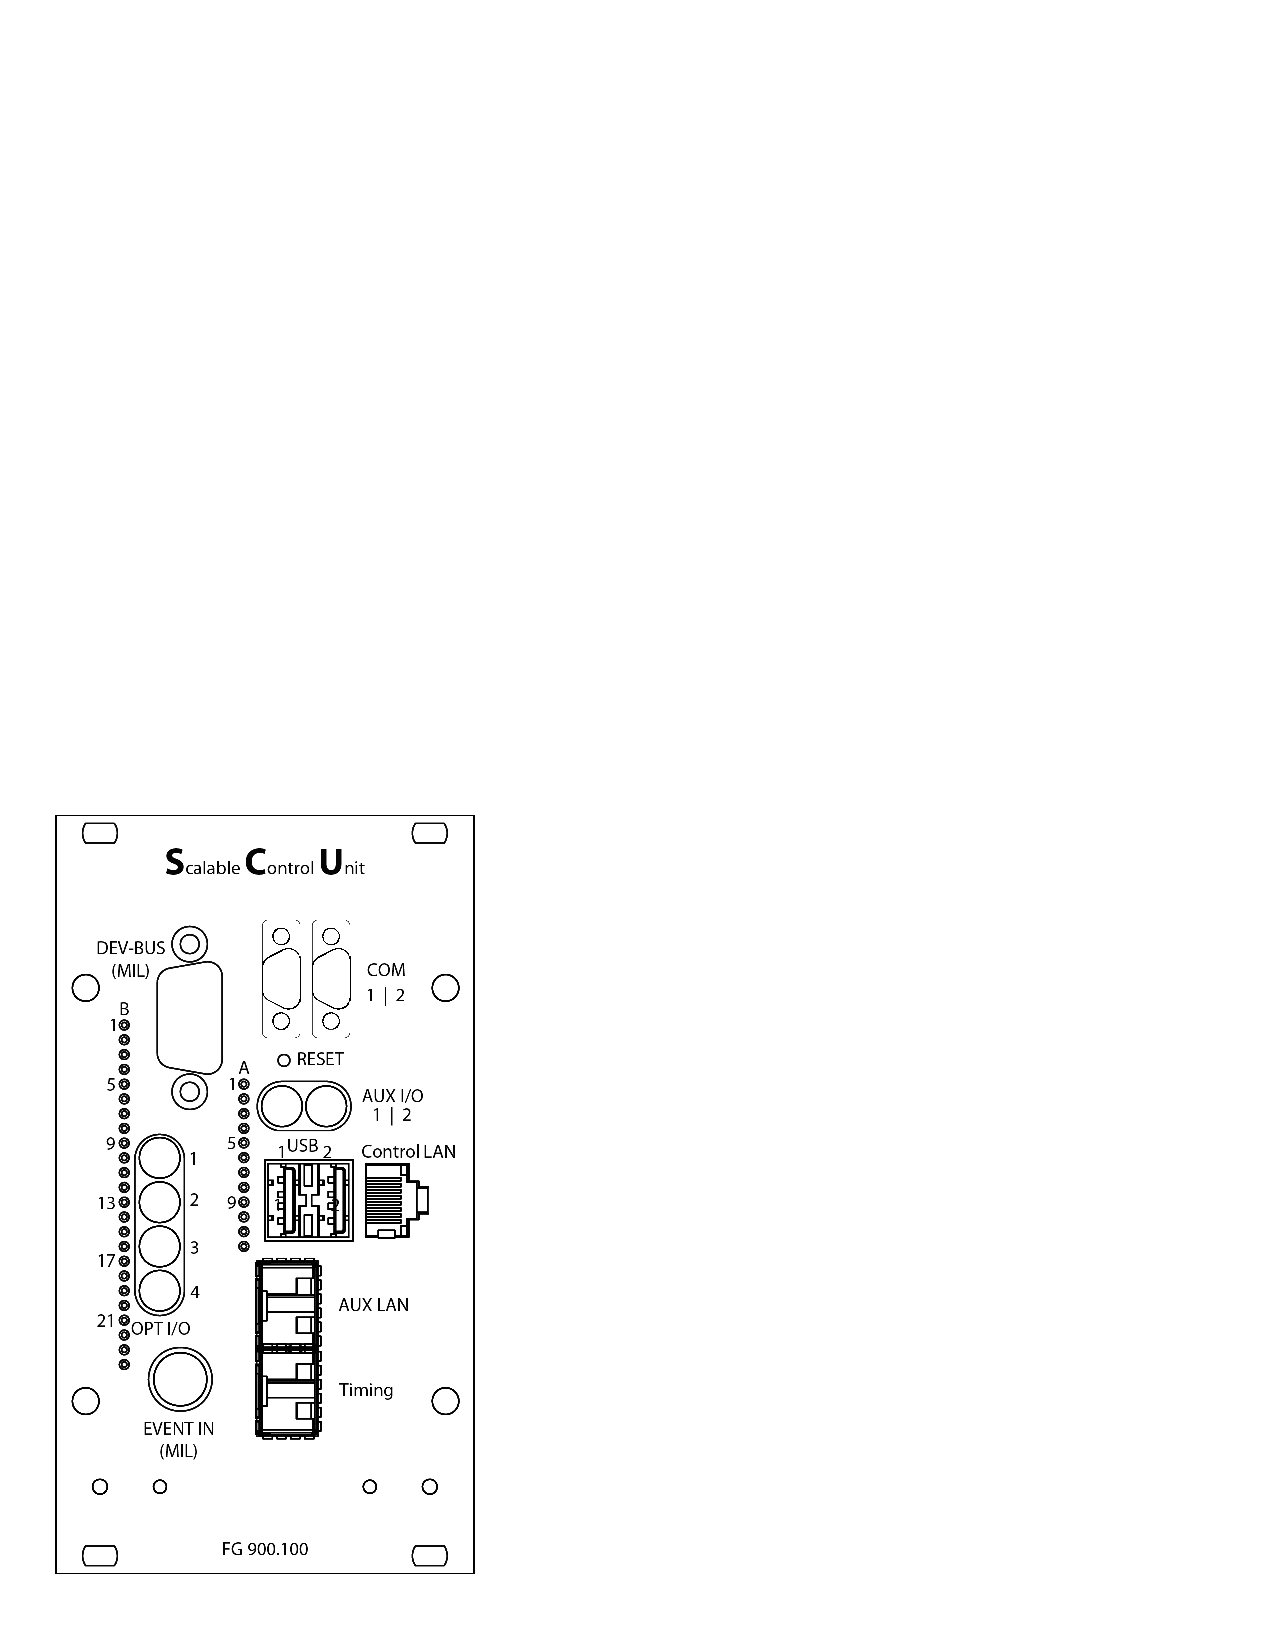
\includegraphics[width=0.49\columnwidth]{../images/WEPMN018f3}}
%\caption{Gesamtbild-Unterschrift}
%\end{figure}

%\begin{minipage}[hbt]{0.5\columnwidth}
%	\centering
%	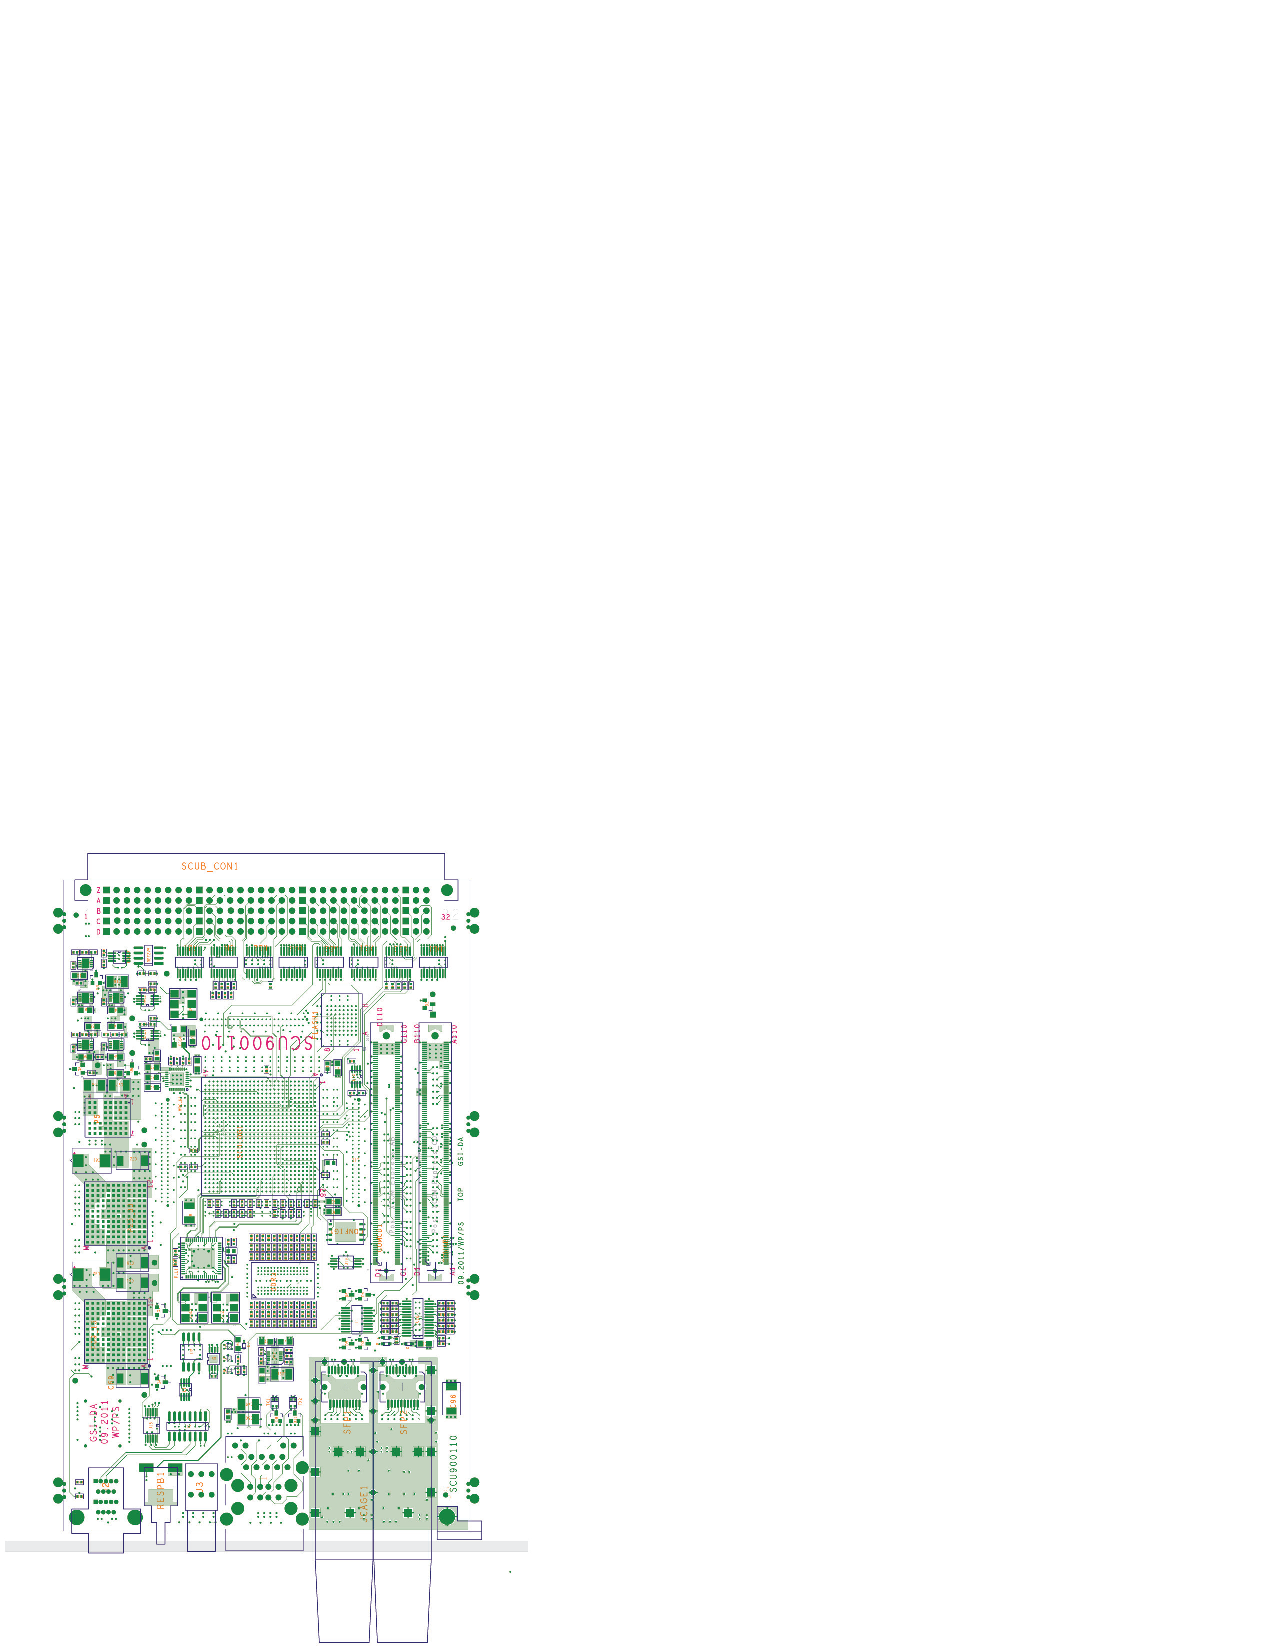
\includegraphics[width=0.49\columnwidth]{../images/WEPMN018f2}
%	\caption{Carrier Board Layout}
%	\label{Bild2}
%\end{minipage}
%\hfill
%\begin{minipage}[hbt]{0.49\columnwidth}
%	\centering
%	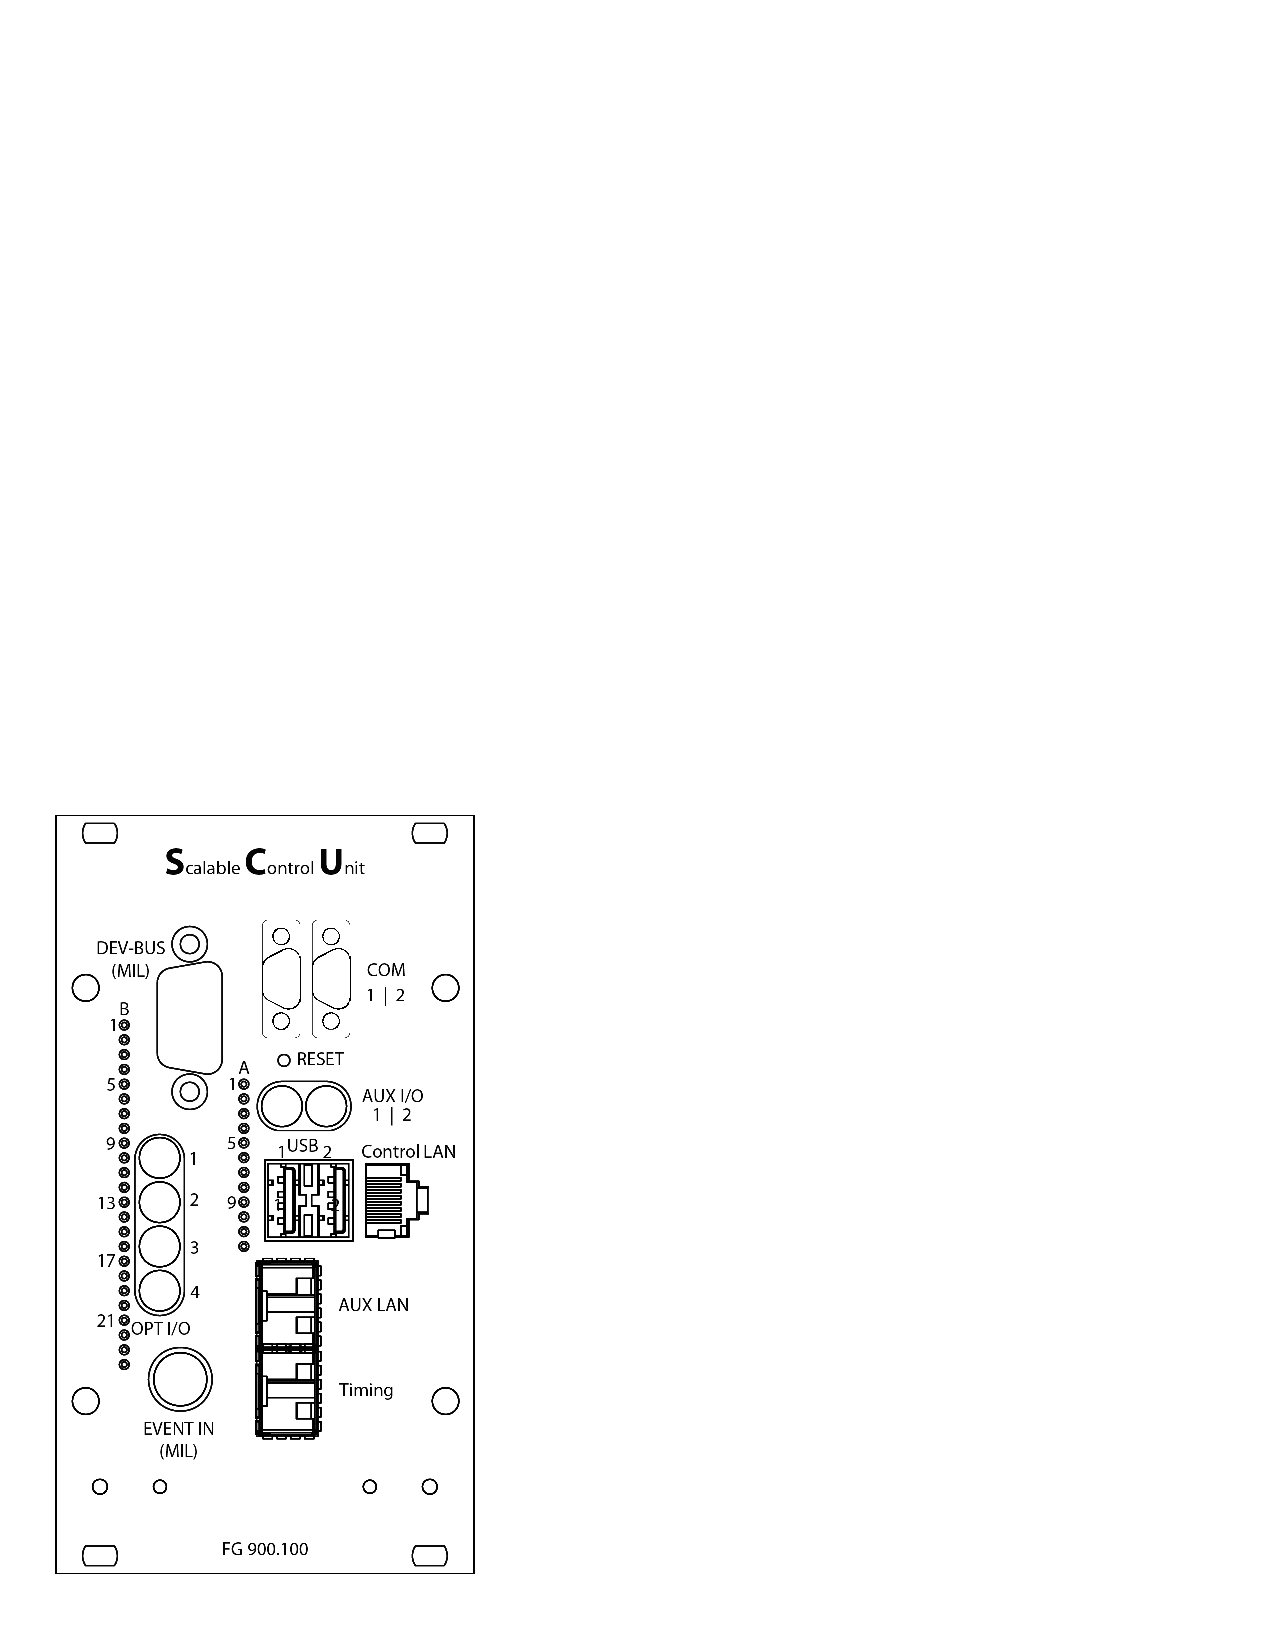
\includegraphics[width=0.49\columnwidth]{../images/WEPMN018f3}
%	\caption{Front Panel}
%	\label{Bild3}
%\end{minipage}

%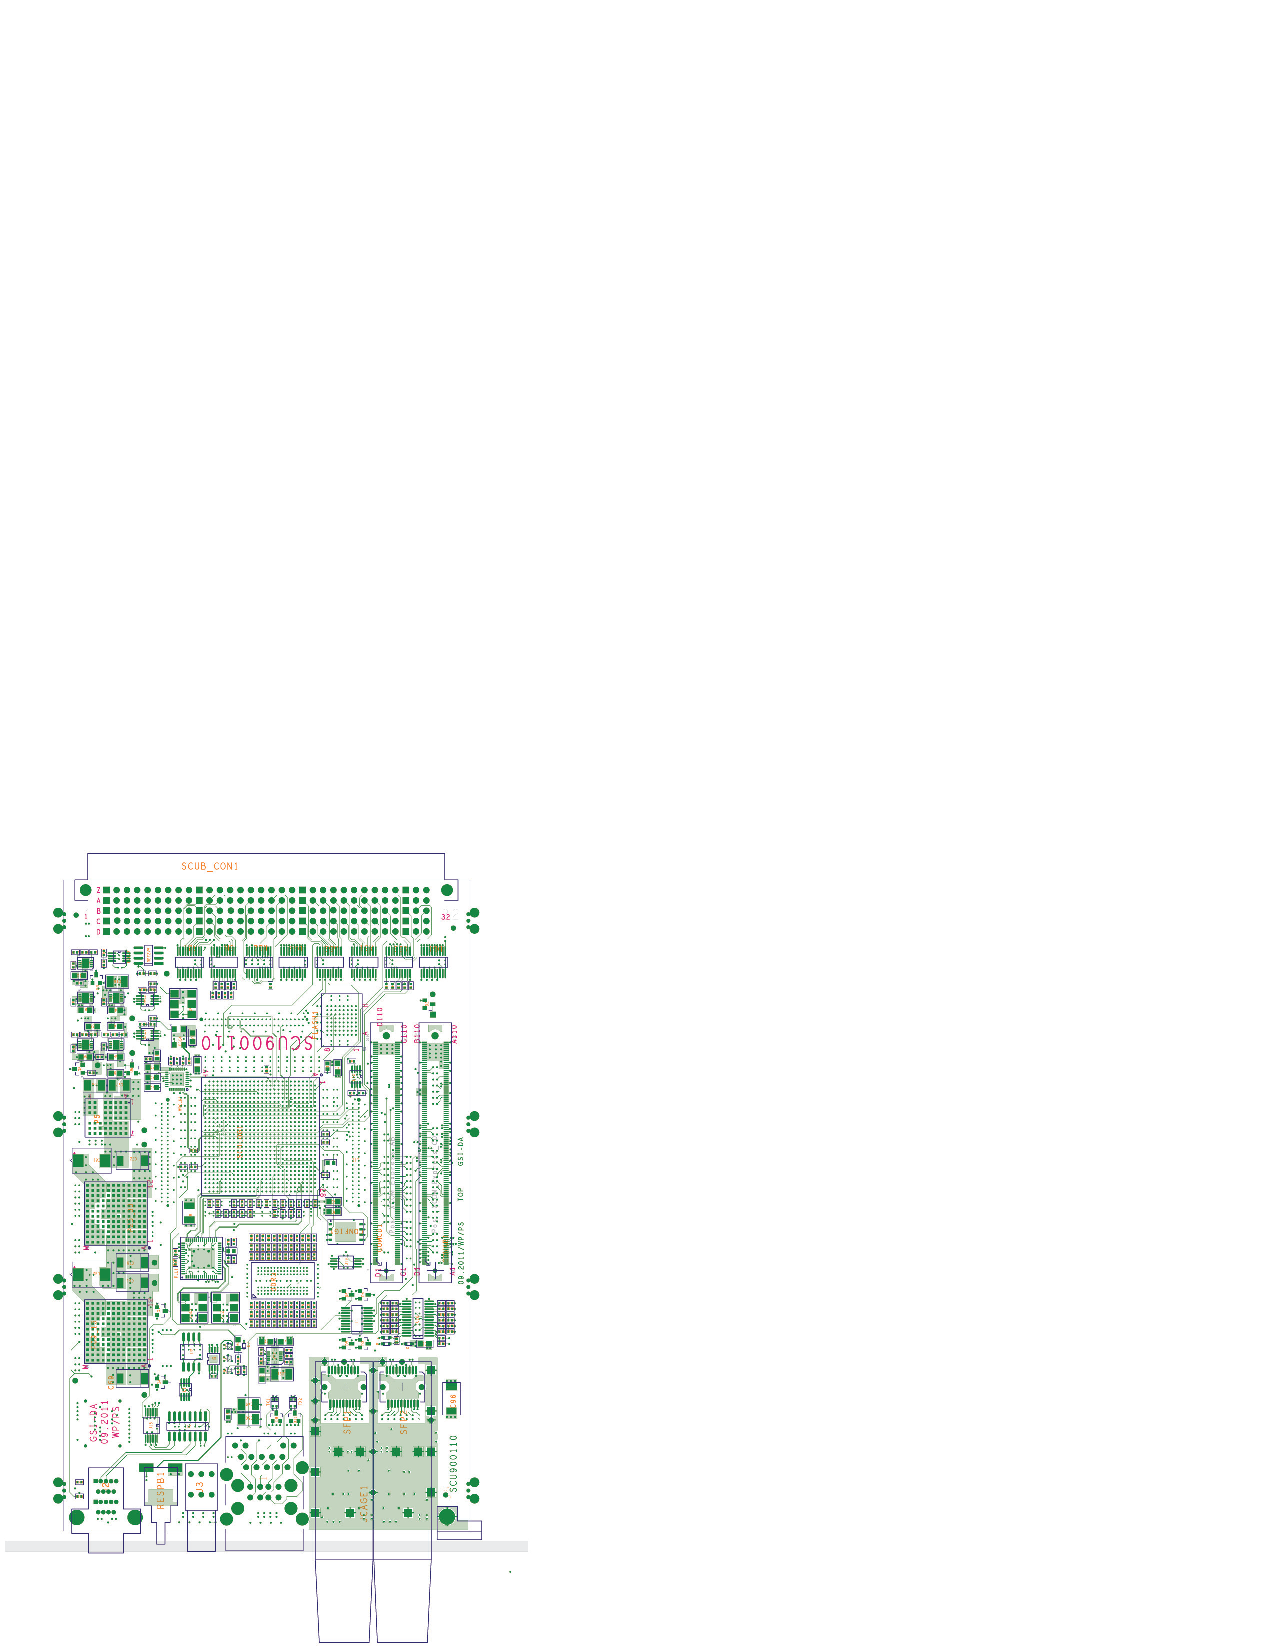
\includegraphics[width=0.49\columnwidth]{../images/WEPMN018f2}
%\captionof{figure}{Layout of the SCU Carrier Board}
\section{Problems during design phase}
\begin{itemize}
	\item fitting of high speed serial transceivers
	\item timing issues with DDR3 memory controller
\end{itemize}

\section{Lessons Learned}
\begin{itemize}
	\item plan a lot more time for testing new technologies
	\item most changes cannot be made after PCB is finished
\end{itemize}


\section{In Detail: Implementing a LPC UART}
\begin{itemize}
	\item Problem: SuperIO Chip does not fit in Layout
	\item Solution: extending LPC bus to FPGA, implementing UART functionality in logic
\end{itemize}


\section{Conclusion}
The measured times as presented in Figure ~\ref{tab:stat_table}
must be reviewed in the context of different use-cases. As an example,
ramping of magnets must be done synchronously. Here, a guaranteed
synchronicity of 10-20$\mu$s must be achieved for ring machines like the
SIS18 and the SIS100. Another example is the control of kicker magnets,
which requires  at least 3ns precision and can only be done with FPGA
Hardware Description Language (HDL). Software on the COM Express module
may only be used for cases, where hard real-time is not required.
As can be seen from the differences of mininum and maximum values, none
of the solutions involving the CPU on the COM Express module fulfill
those requirements, as long as the use of real-time Linux as operating
systems is a stringent requirement for software tools like FESA.

For hard real-time the options are FPGA HDL or LM32 software. Here, FPGA
HDL provides nanoseconds timing while LM32 software provides a better
flexibility. To avoid stringent limitations for future developments of
the FAIR accelerator complex, standard FAIR equipment controllers like
the SCU should be designed supporting hard real-time on the nanoseconds
scale. If flexibility during runtime is required, the ideal solution
could be a combination of both options, where LM32 software creates the
action patterns that are phase aligned with high precision by FPGA HDL.


\vfill

\end{multicols*}
\end{document}
